\documentclass[14pt, fleqn, xcolor={dvipsnames, table}]{beamer}
\usepackage[T2A]{fontenc}
\usepackage[utf8]{inputenc}
\usepackage[english,russian]{babel}
\usepackage{amssymb,amsfonts,amsmath,mathtext}
\usepackage{cite,enumerate,float,indentfirst}
\usepackage{cancel}

\usepackage{tikz}                   
\usetikzlibrary{shadows}

% \usepackage{enumitem}
% \setitemize{label=\usebeamerfont*{itemize item}%
%   \usebeamercolor[fg]{itemize item}
%   \usebeamertemplate{itemize item}}

\graphicspath{{images/}}

\usetheme{Madrid}
\usecolortheme{seahorse}
\renewcommand{\CancelColor}{\color{red}}

\setbeamercolor{footline}{fg=Blue!50}
\setbeamertemplate{footline}{
  \leavevmode%
  \hbox{%
  \begin{beamercolorbox}[wd=.333333\paperwidth,ht=2.25ex,dp=1ex,center]{}%
    И. Кураленок, Н. Поваров, Яндекс
  \end{beamercolorbox}%
  \begin{beamercolorbox}[wd=.333333\paperwidth,ht=2.25ex,dp=1ex,center]{}%
    Санкт-Петербург, 2013
  \end{beamercolorbox}%
  \begin{beamercolorbox}[wd=.333333\paperwidth,ht=2.25ex,dp=1ex,right]{}%
  Стр. \insertframenumber{} из \inserttotalframenumber \hspace*{2ex}
  \end{beamercolorbox}}%
  \vskip0pt%
}
\newcommand\indentdisplays[1]{%
     \everydisplay{\addtolength\displayindent{#1}%
     \addtolength\displaywidth{-#1}}}
\newcommand{\itemi}{\item[\checkmark]}

\title{Линейные модели: жатые чувства, SVM (начнем)\\\small{}}
\author[]{\small{%
И.~Куралёнок,
Н.~Поваров}}
\date{}

\begin{document}

\begin{frame}

\maketitle
\small
\begin{center}
\vspace{-60pt}
\normalsize {\color{red}Я}ндекс \\
\vspace{80pt}
\footnotesize СПб, 2013
\end{center}
\end{frame}
\section{Постановка задачи восстановления сигнала}
\subsection{Пример}
\begin{frame}{Пример}
Сергей Юрьевич любит смотреть телевизор и рассуждать. Есть мнение, что в основном по телевизору "льют воду".
Надо понять как часто надо обращать внимание на то, что проиходит на экране, чтобы не упустить "нить".
\end{frame}
\begin{frame}{Пример: постановка задачи}
\begin{center}
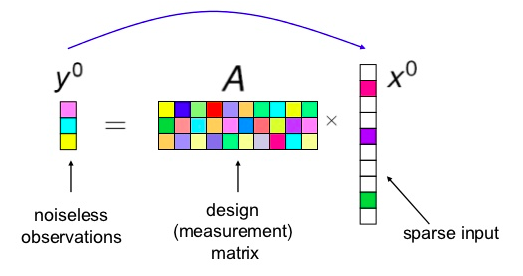
\includegraphics[width=0.7\textwidth]{CS-ProblemSetup-1.png}
\end{center}
\vspace{-1em}
\small
\begin{itemize}
  \item Хотим восстановить сигнал $x^0$
  \item Хотим как можно меньше ``смотреть в телевизор''
  \item Матрица $A$ в данном случате --- то, что происходит в голове Сергея Юрьевича
\end{itemize}
\footnotesize Картинка из Tutorial ICML2010 by Irina Rish \& Genady Grabarnik
\end{frame}

\begin{frame}{Сюрприз compressed sensing}
\small
$$
y = X\beta + \epsilon
$$
Если компоненты матрицы $X$ независимые, одинаково распределенные, нормальные, то $\beta$ можно восстановить точно с большой вероятностью:
\begin{itemize}
  \item из $O(k log(\frac{m}{k}))$ измерений;
  \item решив оптимизацию
    $$\begin{array}{l}
    \arg \min_\beta\|\beta\|_1\\
    \|y - X\beta\| < \epsilon
    \end{array}$$
\end{itemize}
$\Rightarrow$ где-то мы уже такое видели
\end{frame}

\begin{frame}{Линейная регрессия vs. восстановление сигнала}
\begin{itemize}
  \item Решают одну и ту же задачу
  \item Одни и те же алгоритмы
  \item Учиться сложнее:
  \begin{itemize}
    \item нету влияния на построение матрицы $X$;
    \item в частности нет гарантий на свойства матрицы $X$;
    \item наличие в $\beta$ большого количество нулей -- лишь наше предположение.
  \end{itemize}
\end{itemize}
\end{frame}

\subsection{Разложение сигнала в Фурье и постановка в нахождении коэффициентов}
\begin{frame}{Постановка в терминах RFP I}
Нам надо перевести произвольный сигнал (в нашем примере он же во времени!) в линейную комбинацию:
$$\begin{array}{c}
\hat{x_\omega} = \sum_{\omega \in \mathbb{Z}_n} x_j e^{-2\pi i \omega j \over n} \\
\mathcal{F}x = \hat{x}
\end{array}$$
После того как мы все посчитаем в терминах $\hat{x_\omega}$, восстановить телевизор мы сможем по IDFT ($\mathcal{F}^{-1}=\frac{1}{n}\mathcal{F^*}$).
\end{frame}

\section{LASSO для восстановления сигнала}
\begin{frame}{Постановка в терминах RFP II}
  $$\begin{array}{l}
  \arg \min_\beta\|\beta\|_1\\
  y = X\beta
  \end{array}$$
 В новых обозначениях:
$$\begin{array}{l}
\arg \min_\beta \|\beta\|_1 \\
(\mathcal{F}\beta)_k = (\mathcal{F}x)_k, k \in \Omega
\end{array}$$
\end{frame}

\subsection{Теорема о качестве восстановленного сигнала (Candes et al. 2006)}
\begin{frame}{Теорема о качестве восстановленного сигнала для RFP}
\small
\begin{theorem}[Candes et al. (2006)]
\begin{itemize}
\item[] $x\in\mathbb{C}^n : \{i \in \mathbb{Z}_n|x_i \ne 0\} = T \subset \mathbb{Z}_n$ 
\item[] $\Omega \subset \mathbb{Z}_n$ --- одно из равновероятных множеств размера $n$
\item[] зафиксируем точность $B$
\end{itemize}
$\Rightarrow$ c вероятностью $P \ge 1 - O(n^{-B})$ мы можем точно восстановить $x$, если:
$$
\|\Omega\| \ge C^{'}_B|T|\log m
$$
где $C^{'}_B \simeq 23(B + 1)$
\end{theorem}
\end{frame}

\begin{frame}{Выводы из теоремы}
\begin{itemize}
  \item Теорема рассказывает о свойствах случайной DFT проекции
  \item Загаданный вектор $x$ может быть восстановлен:
  \begin{itemize}
    \item с высокой вероятностью
    \item используя LASSO
    \item количество наблюдений пропорционально количеству ненулей в ``загаданном'' сигнале
  \end{itemize}
\end{itemize}
\end{frame}

\begin{frame}{Упрощение рандома}
В теореме $\Omega$ равномерно распределена по всем множествам размера $n$. Такое сложно генерировать. Значительно проще $\Omega^{'}: \forall j \in \mathbb{Z}_n, P(j \in \Omega) = \tau$. \\
$\Rightarrow$ Для таких проекций вероятность восстановить сигнал примерно такая же.
\end{frame}

\subsection{Стабильность решения: RIP, RRfND (Candes et al. 2006)}
\begin{frame}{Стабильно ли решение?}
\small
Интересны два вида ``стабильности'':
\begin{description}
  \item[стабильность:] маленькие изменения в решении при малом изменении в наблюдениях (изменения в загаданном);
  \item[робастность:] устойчивость к шуму в данных (неточно померяли отлик $x$).
\end{description}
Если мы уже решили проблему построения $T$, то решение стабильно:
$$
\hat{\beta} = (\mathcal{F}^*_{T,\Omega}\mathcal{F}_{T,\Omega})^{-1}\mathcal{F}^*_{T,\Omega}y
$$
Из доказательства теоремы о восстановлении сигнала $\mathcal{F}^*_{T,\Omega}\mathcal{F}_{T,\Omega} > \delta E$ c высокой вероятностью при условии на $\Omega$. А вот с робастностью все сложнее...
\end{frame}

\begin{frame}{А что же с произвольно построенным $X$?}
Пока Сергей Юрьевич получал закодированный в Фурье сигнал и раскодировал его обратным Фурье. А что, если кодировани и раскодирование сигнала происходит как-то иначе. Положим, что так:
$$
(\Phi \beta)_\Omega = (\Psi x)_\Omega
$$
В данном случае мы верим в то, что $dim(\Phi)=dim(\Psi)$, более того, будем рассматривать ортонормированные $\Phi, \Psi$

\end{frame}

\begin{frame}{Когерентность базисов}
\small
\begin{definition}
Для пары ортонормальных базисов назовем
$$
\mu(\Phi, \Psi) = \sqrt{n}\max_{i,j} |\phi_i, \psi_j|
$$
\textbf{когерентностью}.
\end{definition}
\begin{itemize}
  \item Заметим, что $1 \le \mu(\Phi,\Psi) \le \sqrt{n}$
  \item В случае Фурье получается экстремально хороший случай: $\mu(DFT,IDFT) = 1$
\end{itemize}
\end{frame}

\begin{frame}{Теорема о качестве восстановленного сигнала для произвольных базисов}
\small
\begin{theorem}[Candes and Romberg (2006)]
Для фиксированной $\delta > 0$ и $x \in \mathbb{R}^n$, $|\{i | x_i \ne 0\}| < S$. Выберем $\Omega$ точек для наблюдения равномерно из $\mathbb{Z}_n$ без повторений. Если
$$|\Omega| \ge C \mu^2(\Phi,\Psi)S\log {n\over\delta}$$
тогда решение LASSO:
$$\begin{array}{l}
\arg \min_{\beta \in \mathbb{R}^n} \|\beta\|_1 \\
(\Phi \beta)_\Omega = (\Psi x)_\Omega
\end{array}$$
восстановит $x$ с вероятностью $1 - \delta$
\end{theorem}
\end{frame}

\subsection{LASSO persistency theorem (Bickel et al., 2009)}
\begin{frame}{Что дальше?}
\small
\begin{enumerate}
  \item Вводим ограничение на модельную матрицу (Restricted Isomenry Property), которое позволяет перейти от условий на модуль образа к условиям на модуль исходного вектора
  \item В введенных условиях получаем ограничение на робастность в рамках восстановления сигнала
  \item Переходим от когерентности к условиям на собственные числа модельной матрицы
\end{enumerate}
В итоге получается, что (LASSO persistency theorem, Bickel et al., 2009):
$$
\|\hat{\beta} - \beta^*\| \le O\left(\sqrt{\log n \over m}\right)
$$
\end{frame}

\begin{frame}{Что мы узнали про CS}
\small
\begin{enumerate}
  \item Можно ставить задачу по восстановлению сигнала
  \item Для решения задачи нам понадобится рандомно выбирать точки наблюдения
  \item Оказывается, что решать подобные задачи нужно тем же самым LASSO
  \item Эффективность решения зависит от того, как построить ``язык передачи информации''
  \item Одним из самых хороших универсальных языков (c минимально возможной когерентностью) является DFT/IDFT
  \item C помощью механизма CS можно доказать устойчивость решения LASSO
\end{enumerate}
\end{frame}

\section{Support vector machines}
\subsection{Идея метода}
\begin{frame}{SVM(воспоминания о былом)}
\begin{itemize}
  \item Последний из линейных методов, который мы рассмотрим подробно.
  \item Rocket science до конца 90-х, по крайней мере в задачах классификации.
\end{itemize}
\end{frame}

\begin{frame}{SVM на пальцах}
\begin{itemize}
  \item Максимальный зазор.
  \item Нелинейные преобразования.
\end{itemize}
\begin{center}
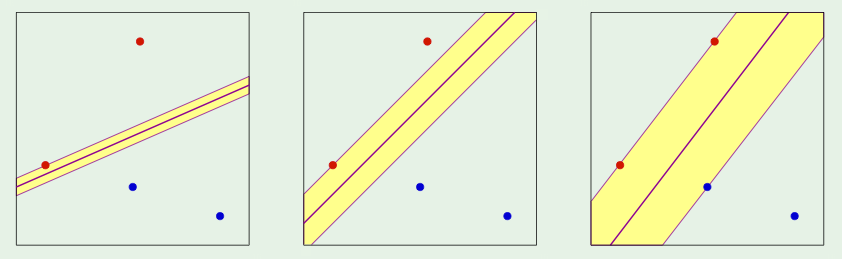
\includegraphics[width=0.9\textwidth]{SVM_1.png}
\end{center}
\end{frame}

\begin{frame}{Мысли вслух}
\begin{itemize}
  \item Почему большой зазор это хорошо?
  \item Какая $\beta$ максимизирует зазор? 
\end{itemize}
\end{frame}

\begin{frame}{Найдем ширину ``зазора'': геометрия}
\small
Есть две параллельные плоскости:
$$\left\{\begin{array}{l}
\beta^T x = a \\
\beta^T x = b
\end{array}\right.$$
проведем прямую, перпендикулярную этой плоскости: $y=\|\beta\| \frac{\beta}{\|\beta\|} t$. Пересечет она наши плоскости вот так:
$$\left\{\begin{array}{l}
\beta^T (\|\beta\| \frac{\beta}{\|\beta\|} t_a) = a \\
\beta^T (\|\beta\| \frac{\beta}{\|\beta\|} t_b) = b
\end{array}\right.$$
$$\left\{\begin{array}{l}
t_a = \frac{a}{\|\beta\|} \\
t_b = \frac{b}{\|\beta\|}
\end{array}\right.$$
тогда расстояние по полученной прямой: $|t_a - t_b| = \frac{|a-b|}{\|\beta\|}$ 
\end{frame}

\begin{frame}{Найдем ширину ``зазора'': мат. анализ}
\footnotesize
Решим оптимизацией:
$$
\min \frac{1}{2}\|x - y\|^2
$$
$$\left\{\begin{array}{l}
\beta^T x = a \\
\beta^T y = b
\end{array}\right.
$$
Перейдем к коэффициентам Лагранжа:
$$
\min \frac{1}{2}\|x - y\|^2 + \lambda_1 (\beta^Tx - a) + \lambda_2 (\beta^Ty - b)
$$
Найдем нули производных по всем переменным:
$$
\begin{array}{lll}
\left\{\begin{array}{l}
\beta^T x = a \\
\beta^T y = b \\ 
x - y + \lambda_1 \beta = 0 \\
x - y + \lambda_2 \beta = 0 \\
\end{array}\right.
&
\left\{\begin{array}{l}
\beta^T(x - y) = a - b \\
\lambda_1 = \lambda_2 \\
\|\beta\|\lambda_1 = b - a \\
\end{array}\right.
&
\left\{\begin{array}{l}
\lambda_1 = \lambda_2 = \frac{b-a}{\|\beta\|^2} \\
x - y = \frac{b - a}{\|\beta\|^2}\|\beta\|\left(\frac{\beta}{\|\beta\|}\right)
\end{array}\right.
\end{array}$$
\end{frame}

\begin{frame}{Возвращаясь к SVM}
\small
Теперь мы знаем что оптимизировать. Отнормируем разделяющие плоскости так:
$$
\left\{\begin{array}{l}
\beta^T x = b - 1 \\
\beta^T x = b + 1 \\
\end{array}\right.
$$
В этих терминах нас $|a - b|$ фиксированы и оптимизировать мы будем только $\beta$:
$$
\arg \min \frac{\|\beta\|}{2}
$$
Вот в таких условиях ($y_i \in \{-1,1\}$):
$$%\left\{
\begin{array}{l}
y_i(\beta^T x_i - b) \ge 1
\end{array}
%\right.$$
$$
\end{frame}

\subsection{Коэффициенты Лагранжа для решения задачи про максимальное расстояние}
\begin{frame}{По методу Лагранжа}
По теореме Куна-Таккера: \
$$
\mathcal{L} = \frac{1}{2}\|\beta\|^2 - \sum_{i=1}^m\lambda_i(y_i(\beta x_i - \beta_0) - 1), \lambda_i \ge 0
$$ 
$$
\left\{  
           \begin{array}{ll}  
            -\mathcal{L} = -\sum_{i=1}^m\lambda_i + \frac{1}{2}\sum_{i=1}^m\sum_{j=1}^m\lambda_i\lambda_j y_i y_j (x_i x_j) \\  
            \lambda_i \ge 0 & \\
            \sum_{i=1}^m\lambda_i y_i = 0
           \end{array}   
           \right.
$$
Тогда: \
$$\begin{array}{l}
\beta = \sum_{i=1}^m\lambda_i y_i x_i \\
\beta_0 = \beta x_i - y_i, \lambda_i > 0
\end{array}$$
\end{frame}

\begin{frame}{Чем стало легче?}
\begin{itemize}
  \item Адовые условия сменились простым $\lambda_i > 0$
  \item У нас получился квадрат количества точек
  \item Интересны только $(x_i, x_j)$ с которыми мы можем играться (kernel trick)!
\end{itemize}
\end{frame}

\subsection{Переход к дуальному решению}
\subsection{Идея как можно на халяву это решить}
\subsection{Kernel trick}
\subsection{Сведение SVM к регуляризации (основная идея)}
\subsection{Домашнее задание}
\begin{frame}{Результаты ДЗ четвёртой недели}
\tiny
\begin{center}
\begin{enumerate}
\item ca876
\item 3fc89
\item e46c8
\item 76a61
\item 165f4
\item 729da
\item cd90b
\item cdb5c
\item 23449
\item c8b18
\item 5660e
\item 257d3
\item 2431e
\item 346a9
\item 6f1ba
\item ab851
\item 3ebe0
\item 49dd1
\item 1938b
\end{enumerate}
\end{center}
\end{frame}

\begin{frame}{Интерпретация результатов}
Задача была придумать несколько таргетов.
\begin{center}
\begin{itemize}
\item 1 место - очень круто;
\item 2 место - почти очень круто;
\item 3-4 места - знают, что такое целевая функция, помнят про "бесконечные потери";
\item 5-10 места - знают, что такое целевая функция, но местами забыли про "бесконечные потери";
\item 11-12 места - знают, что такое целевая функция, но забыли про "бесконечные потери" совсем;
\item 13-19 места - перепутали целевую функцию с решающей, а особо отличившиеся с факторами.
\end{itemize}
\end{center}
\end{frame}

\begin{frame}{Домашнее задание}
\begin{itemize}
\item датасет тот же;
\item сегодня узнали про новые методы - будем применять;
\item howto.txt;
\item дедлайн - 29 ноября.
\end{itemize}
\end{frame}

\end{document}
